%%%%%%%%%%%%%%%%%%%%%%%%%%%%%%%%%%%%%%%%%
% University/School Laboratory Report
% LaTeX Template
% Version 3.1 (25/3/14)
%
% This template has been downloaded from:
% http://www.LaTeXTemplates.com
%
% Original author:
% Linux and Unix Users Group at Virginia Tech Wiki 
% (https://vtluug.org/wiki/Example_LaTeX_chem_lab_report)
%
% License:
% CC BY-NC-SA 3.0 (http://creativecommons.org/licenses/by-nc-sa/3.0/)
%
%%%%%%%%%%%%%%%%%%%%%%%%%%%%%%%%%%%%%%%%%

%----------------------------------------------------------------------------------------
%	PACKAGES AND DOCUMENT CONFIGURATIONS
%----------------------------------------------------------------------------------------

\documentclass{article}
\usepackage{graphicx}
\usepackage{subcaption}
\usepackage{wrapfig}
\graphicspath{ {.} }
\usepackage{listings}
\usepackage{multirow}
\renewcommand\thesubsection{\arabic{subsection}}
\renewcommand\thesubsubsection{\alph{subsubsection}}
\usepackage[justification=centering]{caption}
\usepackage{booktabs}
\usepackage{hyperref}
\hypersetup{
    colorlinks=true,
    linkcolor=blue,
    filecolor=magenta,      
    urlcolor=blue,
}
\usepackage[margin=1.5in]{geometry}
\usepackage{float}
\usepackage{array}
\usepackage{adjustbox}
\newcolumntype{C}[1]{>{\centering\let\newline\\\arraybackslash\hspace{0pt}}m{#1}}


%----------------------------------------------------------------------------------------
%	DOCUMENT INFORMATION
%----------------------------------------------------------------------------------------

\title{CS 6241: Compiler Design \\~\\ Solving Constant Propagation Data-flow Problem Using Detected Destructive Merges Information} % Title

\author{Chayne \textsc{Thrash} and Mansour \textsc{Alharthi}} % Author name

\date{\today} % Date for the report

\begin{document}

\maketitle % Insert the title, author and date

\begin{center}
\begin{tabular}{l r}
Instructor: & Professor Santosh \textsc{Pande} % Instructor/supervisor
\end{tabular}
\end{center}

\subsection{Introduction}
In this project, we implemented the algorithm introduced in paper "Comprehensive Path-sensitive Data-flow Analysis" by Thakur and Govindarajan. The algorithm first detects the nodes where two or more paths merge; causing constant variables defined in one or more of those paths no longer feasible for propagating. After that, the algorithm look for the influenced nodes; the nodes of which will be optimized in case the destructive merge is eliminated. Finally, the algorithm duplicates the nodes that are in the \textit{region of influence}, and thus eliminating the destructive merge allowing for the constant propagation to the influenced nodes. The algorithm represents a trade-off between code size and data-flow precision. We apply the algorithm on only the two top fittest destructive merges, as per the definition of fitness in the paper. 

\subsection{Test Results}
We tested our implementation on two benchmarks. We compare our implementation with sparse conditional constant propagation technique by Wegman-Zadeck implemented in LLVM. 

~\\~

\begin{adjustbox}{center}
\renewcommand{\arraystretch}{2}
%\begin{table}[]
\begin{tabular}{| C{3cm} | C{3cm} | C{3cm} | C{3cm} | C{3cm} |}
\hline
Benchmark & Static size with sparse conditional constant propagation & Static size with destructive merge elimination & \% of increase in static size \\ \cline{1-4} 
bzip2 & 88776B & 105160B & \%18  \\ \cline{1-4}
gzip & 77584B & 85776B & \%11  \\ \cline{1-4}
\end{tabular}
%\end{table}
\end{adjustbox}
\captionof{table}{Static size comparison} 


\begin{adjustbox}{center}
\renewcommand{\arraystretch}{2}
%\begin{table}[]
\begin{tabular}{| C{3cm} | C{3cm} | C{3cm} | C{3cm} | C{3cm} |}
\hline
Benchmark & Constants propagated\# with sparse conditional constant propagation & Constants propagated\# with destructive merge elimination & \% of Constants propagated increased \\ \cline{1-4} 
bzip2 & 56 & 107 & \%91  \\ \cline{1-4}
gzip & 31 & 106 &  \%240 \\ \cline{1-4}

\end{tabular}
%\end{table}
\end{adjustbox}
\captionof{table}{Constants propagated comparison} 

~\\~
\begin{adjustbox}{center}
\renewcommand{\arraystretch}{2}
%\begin{table}[]
\begin{tabular}{| C{4cm} | C{3cm} | C{3cm} | C{3cm} | C{3cm} |}
\hline
Benchmark & Execution time with sparse conditional constant propagation & Execution time with destructive merge elimination & \% of change in Execution time \\ \cline{1-4} 
bzip2 & 0.357s & 0.909s & \%154  \\ \cline{1-4}
gzip  & 0.073s & 0.176s & \%150  \\ \cline{1-4}
\end{tabular}
%\end{table}
\end{adjustbox}
\captionof{table}{Execution time comparison when a compressing 1.2MB file} 

~\\~

Figures 1 and 2 show examples of a function CFG with SCCP and Destructive merges transformations. The function is taken from the bzip2 benchmark codebase. This example shows the elimination of the PHI function in the return block by splitting the path resulting in the propagation of the returned values all the way to the exit points. 

\begin{figure}[H]
\begin{subfigure}{1\textwidth}
  \centering
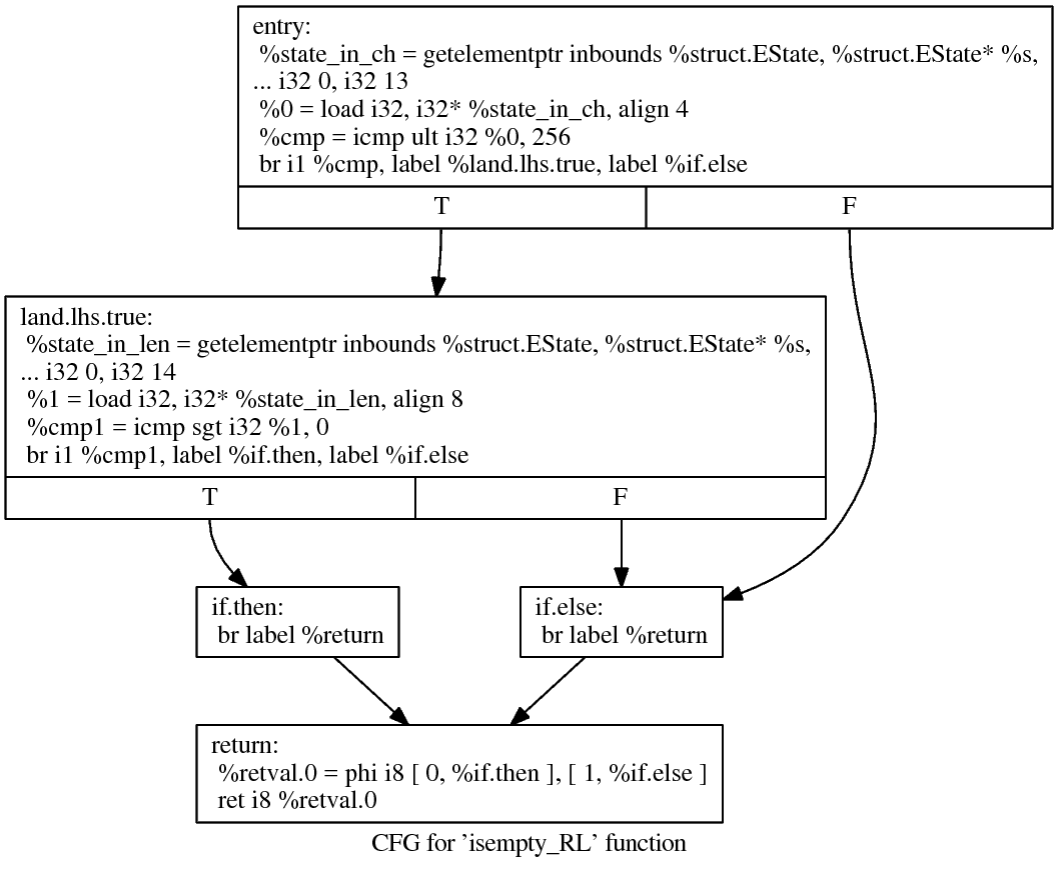
\includegraphics[width=300px]{bzip2-example-sccp} 
\end{subfigure}
\caption{function isempty\_RL in bzip2 with SCCP transformation}
\label{fig:test}
\end{figure}

\begin{figure}[H]
\begin{subfigure}{1\textwidth}
  \centering
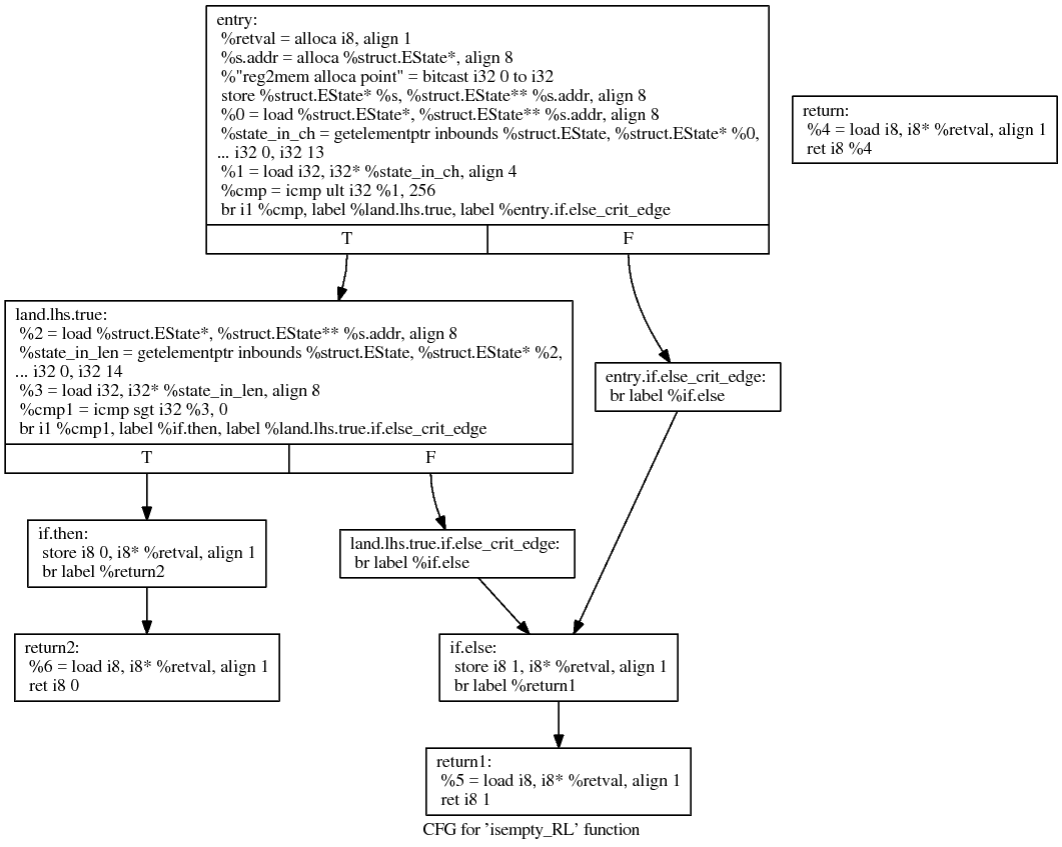
\includegraphics[width=280px]{bzip2-example-dm} 
\end{subfigure}%
\caption{function isempty\_RL in bzip2 with Destructive merge transformation}
\label{fig:test}
\end{figure}


\subsection{Work Breakdown}
~\\~
\begin{adjustbox}{center}
\renewcommand{\arraystretch}{2}
%\begin{table}[]
\begin{tabular}{| C{3cm} | C{3cm} | C{3cm} | C{3cm} | C{3cm} |}
\hline
Destructive Merges Detection & Split Graph and CFG Reconstruction & Preliminary Reachability Analysis & Report & Integrating and testing \\ \cline{1-5} 
Mansour & Chayne & Chayne & Mansour &  Chayne\&Mansour \\ \cline{1-5}

\end{tabular}
%\end{table}
\end{adjustbox}
\captionof{table}{breakdown of work among team members} 

\end{document}